\documentclass[11pt]{article}
\usepackage[margin=2.2cm]{geometry}
\usepackage{amsmath,amssymb,xcolor}
\setlength{\parindent}{0pt}\setlength{\parskip}{7pt}
\usepackage[compat=1.1.0]{tikz-feynman}
\tikzfeynmanset{every photon={/tikz/decoration={snake,amplitude=1.1pt,segment length=4pt}}}
\newcommand{\Fsq}{F_{\mu\nu}F^{\mu\nu}}
\begin{document}
\begin{center}
{\Large $\gamma\gamma\to\phi\phi$ through the charged-meson loop}
\end{center}

\section*{1. Setup}
We need the part of the lowest-order $\chi$PT Lagrangian that couples $\phi$
and photons to the charged mesons. For each charged meson $j=\pi^+,K^+$ this is
just scalar QED with an extra mass-like term from $\phi$:
\begin{equation}
  \mathcal L \supset |D_\mu\pi_j|^2 - m_j^2\,|\pi_j|^2 - \mu_j\,\phi\,|\pi_j|^2,
  \qquad \mu_\pi = B_0(g_u+g_d),\quad \mu_K = B_0(g_u+g_s).
\end{equation}
The scalar $\phi$ enters $\chi$PT through the quark-mass matrix,
$M_q\to M_q+g\phi$, and the $\chi$PT mass term is \emph{linear} in $M_q$. So
$\phi$ appears only linearly: there is no $\phi^2|\pi|^2$ contact term at this
order. This has a useful consequence. If we treat $\phi$ as a constant
background field, the meson mass it produces is exactly
\begin{equation}
  M_j^2(\phi) = m_j^2 + \mu_j\,\phi ,
\end{equation}
with no higher powers of $\phi$.

\section*{2. Which diagrams contribute}
We want the amplitude at order $e^2\mu^2$, with both photons and both $\phi$'s
attached to a single meson loop. Two classes of diagram do this:
\begin{itemize}\itemsep2pt
  \item \textbf{boxes:} four three-point vertices on the loop (two
        $\gamma\pi\pi$, two $\phi\pi\pi$), in all orderings around the loop;
  \item \textbf{triangles:} the two photons enter together through the seagull
        $2ie^2g^{\mu\nu}$, and the two $\phi$'s through separate $\phi\pi\pi$
        vertices.
\end{itemize}
\begin{center}
\begin{tabular}{ccc}
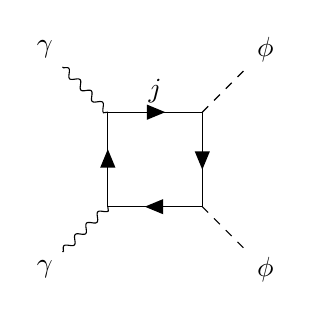
\begin{tikzpicture}[baseline=(c)]
\begin{feynman}
\vertex (a) at (0,1.2); \vertex (b) at (1.2,1.2);
\vertex (c) at (1.2,0); \vertex (d) at (0,0);
\vertex (g1) at (-0.8,2.0) {$\gamma$}; \vertex (g2) at (-0.8,-0.8) {$\gamma$};
\vertex (p1) at (2.0,2.0) {$\phi$};  \vertex (p2) at (2.0,-0.8) {$\phi$};
\diagram*{
 (g1) -- [photon] (a), (g2) -- [photon] (d),
 (b) -- [scalar] (p1), (c) -- [scalar] (p2),
 (a) -- [fermion, edge label=$j$] (b) -- [fermion] (c) -- [fermion] (d) -- [fermion] (a),
};
\end{feynman}
\end{tikzpicture}
&\qquad
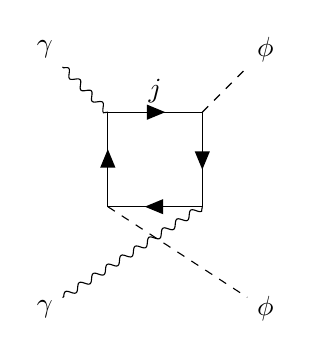
\begin{tikzpicture}[baseline=(c)]
\begin{feynman}
\vertex (a) at (0,1.2); \vertex (b) at (1.2,1.2);
\vertex (c) at (1.2,0); \vertex (d) at (0,0);
\vertex (g1) at (-0.8,2.0) {$\gamma$}; \vertex (g2) at (-0.8,-1.3) {$\gamma$};
\vertex (p1) at (2.0,2.0) {$\phi$};  \vertex (p2) at (2.0,-1.3) {$\phi$};
\diagram*{
 (g1) -- [photon] (a), (g2) -- [photon] (c),
 (b) -- [scalar] (p1), (d) -- [scalar] (p2),
 (a) -- [fermion, edge label=$j$] (b) -- [fermion] (c) -- [fermion] (d) -- [fermion] (a),
};
\end{feynman}
\end{tikzpicture}
&\qquad
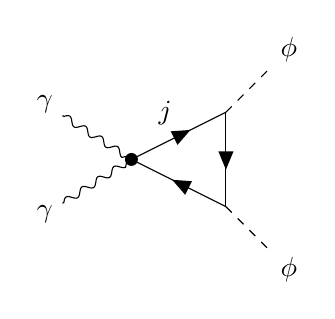
\begin{tikzpicture}[baseline=(c)]
\begin{feynman}
\vertex[dot] (s) at (0,0.6) {}; \vertex (b) at (1.2,1.2); \vertex (c) at (1.2,0);
\vertex (g1) at (-1.1,1.3) {$\gamma$}; \vertex (g2) at (-1.1,-0.1) {$\gamma$};
\vertex (p1) at (2.0,2.0) {$\phi$};  \vertex (p2) at (2.0,-0.8) {$\phi$};
\diagram*{
 (g1) -- [photon] (s), (g2) -- [photon] (s),
 (b) -- [scalar] (p1), (c) -- [scalar] (p2),
 (s) -- [fermion, edge label=$j$] (b) -- [fermion] (c) -- [fermion] (s),
};
\end{feynman}
\end{tikzpicture}
\\[4pt]
(a) box, photons adjacent & (b) crossed box & (c) seagull triangle
\end{tabular}
\end{center}
{\small Solid lines are the charged meson $j=\pi^+,K^+$ (arrow = charge
flow), dashed lines $\phi$, wavy lines photons. Diagram (a) comes twice
($\phi_1\leftrightarrow\phi_2$); (b) is (a) with a photon and a $\phi$ swapped, so the photons sit on opposite corners of the loop, and every diagram comes with both charge flows;
(a), (b), (c) are the three inequivalent cyclic orderings plus the seagull.}

(A bubble would need either a $\phi\phi\pi\pi$ vertex, which doesn't exist, or
two seagulls, which is order $e^4$.) Neither class is gauge invariant on its
own; only the sum is. Rather than evaluate the loop integrals directly, we use
the fact that for external momenta small compared with the meson mass,
$s,\,m_\phi^2\ll 4m_j^2$, the sum is completely fixed by a low-energy theorem.

\paragraph{Is that everything?} At leading order, yes. The low-energy theorem
below is the full one-loop effective action of the charged mesons in a
background $\phi$, so it sums every one-loop diagram, in every ordering, for
$\pi^+$ and $K^+$ together; nothing has to be enumerated by hand. Nothing else
enters at order $\alpha\mu^2$:
\begin{itemize}\itemsep2pt
  \item neutral mesons ($\pi^0,\eta,K^0$) have no photon coupling at this order;
  \item there is no tree-level contribution: $\phi$ is neutral, the
        $\mathcal O(p^2)$ Lagrangian has no $\phi\phi\gamma\gamma$ contact term,
        and a scalar $\phi$ does not mix with $\pi^0$ or $\eta$ (parity), so
        there is no $t$-channel meson exchange;
  \item exchanging a neutral state between two $\gamma\phi$ vertices needs it
        to be C-odd: a photon (Section~6, order $\alpha^2$) or a $\rho/\omega$,
        which lies outside leading-order $\chi$PT and is suppressed by
        $s/m_\rho^2$;
  \item $s$-channel $\gamma\gamma\to\phi^*\to\phi\phi$ needs a $\phi^3$
        coupling. The model has none at tree level, and the meson-loop one is
        $\propto\mu^3$, i.e.\ higher order in the quark couplings.
\end{itemize}
What is left out is genuinely higher order: two-loop and $\mathcal O(p^6)$
terms, and the $s/m_j^2$, $m_\phi^2/m_j^2$ corrections (Section~7).

\section*{3. The low-energy theorem}
When a charged scalar of mass $M$ is integrated out, its one-loop vacuum
polarisation shifts the photon kinetic term. The size of the shift is set by
the scalar's contribution to the QED $\beta$-function ($b=\tfrac13$, a quarter
of a Dirac fermion's), and for slowly varying fields it reads
\begin{equation}
  \mathcal L_{\rm eff} \supset \frac{e^2}{192\pi^2}\,\ln M^2\;\Fsq
  = \frac{\alpha}{48\pi}\,\ln M^2\;\Fsq .
\end{equation}
The whole $\phi$ dependence now comes from replacing $M^2$ by the
background-field mass $M_j^2(\phi)$ and expanding the logarithm,
\begin{equation}
  \ln(m^2+\mu\phi) = \ln m^2 + \frac{\mu}{m^2}\,\phi - \frac{\mu^2}{2m^4}\,\phi^2 + \dots
\end{equation}
The first-order term is the familiar $\phi\gamma\gamma$ coupling:
\begin{equation}
  \mathcal L_{\phi\gamma\gamma}
     = \frac{\alpha}{48\pi}\sum_j\frac{\mu_j}{m_j^2}\,\phi\,\Fsq
     \equiv \frac{g_{\phi\gamma\gamma}}{4}\,\phi\,\Fsq,
     \qquad g_{\phi\gamma\gamma} = \frac{\alpha}{12\pi}\sum_j\frac{\mu_j}{m_j^2}.
\end{equation}
This is exactly the triangle result from the explicit loop calculation,
$g_{\phi\gamma\gamma} = \frac{\alpha}{4\pi}\sum_j \frac{\mu_j}{m_j^2}A_0(0)$
with $A_0(0)=\tfrac13$, which is what gives $\mathcal D=\tfrac12(B_0X)^2$. That
agreement is the check on the normalisation.

The second-order term is the one we want. It has no free parameters left once
the first-order term is fixed:
\begin{equation}
  \boxed{\;\mathcal L_{\phi\phi\gamma\gamma}
     = c\,\phi^2\,\Fsq,\qquad c = -\frac{\alpha}{96\pi}\,Y,\qquad
     Y \equiv \sum_j\frac{\mu_j^2}{m_j^4}
     = B_0^2\!\left[\frac{(g_u+g_d)^2}{m_\pi^4}+\frac{(g_u+g_s)^2}{m_K^4}\right]\;}
\end{equation}
Two remarks. First, $Y$ is a sum over mesons of \emph{squares}, not the square
of a sum as in $\mathcal D$, because each meson loop contributes its own
$\phi^2$ term. Second, the relative factor $-\tfrac12$ between the $\phi^2$
and $\phi$ coefficients (in units of $\mu/m^2$) is the same pattern as
$hh\gamma\gamma$ versus $h\gamma\gamma$ from a heavy fermion loop.

\section*{4. Amplitude}
Take photons with momenta and polarisations $(k_1,\epsilon_1)$,
$(k_2,\epsilon_2)$. The operator $c\,\phi^2\Fsq$ gives a factor 2 from the two
identical $\phi$'s and a factor 4 from $\Fsq$, so
\begin{equation}
  \mathcal M = 8c\,\big[(k_1\!\cdot k_2)(\epsilon_1\!\cdot\epsilon_2)
             - (k_1\!\cdot\epsilon_2)(k_2\!\cdot\epsilon_1)\big].
\end{equation}
This is transverse by construction ($\epsilon_i\to k_i$ gives zero), as it must
be. Summing over polarisations, the bracket gives
$2(k_1\!\cdot k_2)^2 = s^2/2$, so
\begin{equation}
  \sum_{\rm pol}|\mathcal M|^2 = 32\,c^2 s^2,\qquad
  \overline{|\mathcal M|^2} = \tfrac14\sum_{\rm pol}|\mathcal M|^2 = 8\,c^2 s^2 .
\end{equation}
The same conventions give $\Gamma_{\phi\to\gamma\gamma}=g_{\phi\gamma\gamma}^2m_\phi^3/64\pi$
from the linear term, so the two are normalised consistently.

\section*{5. Cross section}
The amplitude has no angular dependence, so the distribution is isotropic.
Using $\frac{d\sigma}{d\Omega} = \frac{\beta\,\overline{|\mathcal M|^2}}{64\pi^2 s}$
with $\beta=\sqrt{1-4m_\phi^2/s}$, and including a factor $\tfrac12$ for the
identical $\phi\phi$ final state,
\begin{equation}
  \boxed{\;\sigma(\gamma\gamma\to\phi\phi) = \frac{c^2\,s\,\beta}{4\pi}
  = \frac{\alpha^2\,Y^2}{36864\,\pi^3}\;s\,\beta\;}
  \qquad (s,\ m_\phi^2 \ll 4m_\pi^2).
\end{equation}
As a benchmark, for $g=[1\,1\,1]/3$ we get $Y = 9.42\times10^3$ GeV$^{-2}$
(almost entirely from the pion), and
$\sigma \simeq 4.1\times10^{-3}\,\text{GeV}^{-4}\; s\,\beta$.

\section*{6. Comparison with photon exchange}
The other way to make $\phi\phi$ from two photons is $t$- and $u$-channel
photon exchange, with a $\phi\gamma\gamma$ vertex at each end. That amplitude
goes as $g_{\phi\gamma\gamma}^2\sim\alpha^2$, whereas the box is only
$\mathcal O(\alpha)$.
\begin{center}
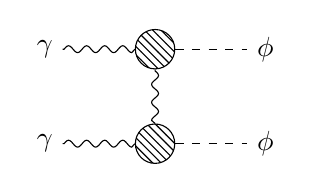
\begin{tikzpicture}
\begin{feynman}
\vertex[blob, minimum size=5mm] (u) at (0,1.2) {}; \vertex[blob, minimum size=5mm] (l) at (0,0) {};
\vertex (g1) at (-1.4,1.2) {$\gamma$}; \vertex (g2) at (-1.4,0) {$\gamma$};
\vertex (p1) at (1.4,1.2) {$\phi$};  \vertex (p2) at (1.4,0) {$\phi$};
\diagram*{
 (g1) -- [photon] (u) -- [scalar] (p1),
 (g2) -- [photon] (l) -- [scalar] (p2),
 (u) -- [photon] (l),
};
\end{feynman}
\end{tikzpicture}
\qquad{\small ($+\ u$-channel; each blob is the $\phi\gamma\gamma$ meson triangle)}
\end{center} For a single meson the ratio of the two coefficients is
\begin{equation}
  \frac{8|c|}{g_{\phi\gamma\gamma}^2}
  = \frac{\alpha\mu^2/(12\pi m^4)}{\alpha^2\mu^2/(144\pi^2 m^4)}
  = \frac{12\pi}{\alpha}\approx 5\times10^{3},
\end{equation}
up to $\mathcal O(1)$ kinematic factors. Concretely, for $g=[1\,1\,1]/3$ and
$m_\phi\to0$, photon exchange gives
$\sigma = \frac{5\,g_{\phi\gamma\gamma}^4}{1024\pi}\,s = 2.6\times10^{-10}\,\text{GeV}^{-4}\,s$,
so the box is larger by about $1.6\times10^{7}$. The interference term is
suppressed relative to the box by the same $\sim\!\alpha$ factor, so the box
alone is an excellent approximation.

\section*{7. Range of validity}
Everything above is leading order in $s/m_j^2$ and $m_\phi^2/m_j^2$. The pion
term, which dominates, therefore needs $\sqrt s\ll 2m_\pi$. For thermal photons
that means $T\ll 50$ MeV, which comfortably covers the $\Delta N_{\rm eff}$
epoch at $T\sim$ MeV. Near and above the $\pi^+\pi^-$ threshold the full box,
with its $s$-, $t$- and $u$-dependent loop functions, would be needed.
\end{document}
